\section{Theory}

The  risk  of  instability in control circuits are caused by the delays. It is
always  necessary to ensure that a system is stable. There exist  some  simple
tuning rules (proposed by Ziegler-Nichols and Chien, Hrones and Reswick)  that
allow us to calculate stable  parameters  for  P,  PI,  and  PID  controllers.


\subsection{Tuning Rules According to Ziegler-Nichols (Oscillation Method)}

This method relies on a plant that can potentially become unstable. That is to
say,  the  plant  must be of higher order such  that  the  phase  crosses  the
\SI{180}{\degree} threshold at some point. If this is the case, then the plant
can be  placed  in a closed loop with a single gain element (P-Controller) and
the gain can be  increased  until  the  system's  output  begins to oscillate.

\begin{figure}[H]
    \centering
    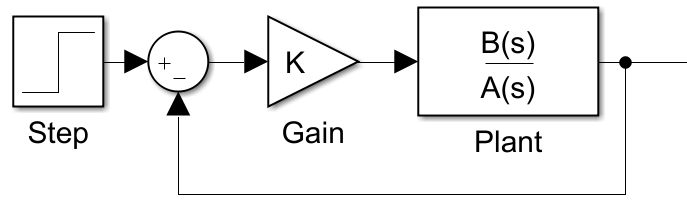
\includegraphics[width=\imagewidth]{images/osc_method.png}
\end{figure}

The gain at which this occurs  is  $K_{p,crit}$  and  the  period  at which it
oscillates is $\tau_{crit}$.

The full procedure of the Ziegler-Nichols method is:

\begin{enumerate}
    \item Use a pure P controller and set a small gain $K_{P}$.
    \item Increasing the gain $K_{P}$ until an undamped oscillation occurs.
    \item Indentify the critical gain $K_{p,crit}$ and the critical period $\tau_{crit}$
    \item According to table \ref{tab:ziegler_nichols} specifying the controllers parameter.
\end{enumerate}

\begin{center}
    \begin{threeparttable}
        \begin{tabular}{cccc}
            \toprule
            Type & $K_{P}$                   &  $T_{i}$                   &  $T_{d}$ \\
            \midrule
            P    &  $0.5  \cdot K_{P,crit}$  &  -                         &  -                         \\
            PI   &  $0.45 \cdot K_{P,crit}$  &  $0.85 \cdot \tau_{crit}$  &  -                         \\
            PID  &  $0.6  \cdot K_{P,crit}$  &  $0.5 \cdot \tau_{crit}$   &  $0.12 \cdot \tau_{crit}$  \\
            \bottomrule
        \end{tabular}
        \caption{Table with controller parameters, according to the Ziegler-Nichols method (good disturbance rejection).}
        \label{tab:ziegler_nichols}
    \end{threeparttable}
\end{center}

The advantage of the Ziegler-Nichols method is  that it is simple to apply and
because of that also easy to understand. On the  other  hand  it is very risky
because the control loop must be operated close to instability.  Dependong  on
the  plant  being  measured  this  can  be  very dangerous and very expensive.

A  disadvantage  is  the  need  for  the  plant to  be  potentially  unstable.
Theoretically not all plants can be made to oscillate in a closed  loop with a
P-controller. The  practical  significance  of  this  method  is thus limited.

